\section{Praktická časť}
\noindent

Praktická časť tejto diplomovej práce sa zaoberá spojením opisovaných častí do jednej softvérovej knižnice pre platformu Arduino Mega 2560. Arduino využíva AVR
architektúru mikrokontrolérov, preto sme značnú časť práce venovali práve štúdiu fungovania týchto mikrokontrolérov.
Jednou z hlavných úloch vytvorenej knižnice je zjednodušenie použitia prerušení s dôrazom na prerušenia časovačov.
Druhou úlohou je modelovanie programu mikrokontroléra pomocou konečných stavových automatov. Spojením týchto dvoch fenoménov sme sa pokúsili zjednodušiť
a zrýchliť vývoj aplikácii aktívne využívajúcich prerušenia mikrokontroléra. Zároveň, knižnica by mala umožniť využitie týchto prerušení aj menej zdatným
používateľom, keďže jej využitie by nemalo vyžadovať hĺbkové znalosti fungovania prerušení na mikrokontroléri Arduino Mega 2560. Knižnicu sme nazvali Interro
a tento názov budeme používať aj neskôr v tejto práci pri opise fungovania a architektúry vytvorenej knižnice. Knižnica je zapísaná v jazyku C++.

\subsection{Architekúra riešenia}
\noindent
Vďaka výberu jazyka C++ sme pri vývoji sme aktívne využívali princípy objektového orientované programovania. Architekúra Interra pozostáva z mnoho vytvorených tried.
Tie je možné rozdeliť na tri hlavné skupiny: Spúšťače, triedy stavového stroja a triedu Interro, ktorá slúži ako globálny kontajner a koordinuje činnosť celej knižnice.
Postupne sa pozrieme na každú túto skupinu a jej úlohy detailnejšie. \par
Pre jednoduchšie porozumenie si vytvorenú knižnicu predstavíme na nasledujúcom jednoduchom príklade: Vytvoríme program, ktorého úlohou je blikanie led žiarovky.
Tá bude meniť svoj stav v 1 sekundovom intervale. Blikanie led žiarovky je možné vypnúť, respektíve zapnúť pomocou stlačenia tlačidla.

\subsubsection{Modelovanie programu pomocou stavového automatu}
\noindent
Prvým krokom každého programu vytvoreného pomocou knižnice Interro je jeho namodelovanie pomocou stavového automatu.
Ako sme spomínali v kapitovale číslo \ref{state-machine-theory}, automat je definovaný päticou ($\Sigma$ ,$\mathcal{Q}$ , $q_0$, $\mathcal{F}$, $\delta$).
Automat označíme ako \textit{P} a začneme definíciou množiny stavov $\mathcal{Q}$. V našom príklade vieme identifikovať 3 stavy:
\begin{enumerate}
    \item Led žiarovka svieti, označme ako \textit{LedOn}.
    \item Led žiarovka nesvieti, označme ako \textit{LedOff}.
    \item Blikanie led žiarovky je vypnuté, označme ako \textit{Idle}.
\end{enumerate}

Pokračujme definíciou vstupnej abecedy $\Sigma$. Túto vstupnú abecedu Interro označuje ako udalosti. V spomínanom príklade je možné definovať tieto udalosti:
\begin{enumerate}
    \item Stlačenie tlačidla, označme ako \textit{ButtonClicked}.
    \item Vypršanie časového intervalu, označme ako \textit{TimeElapsed}.
\end{enumerate}

Nasleduje definícia počiatočného stavu $q_0$. Tým je stav \textit{Idle}. Množina konečných stavov $\mathcal{F}$ je v našom prípade prázdna. Príklad nedefinuje
stav v ktorom má program skončiť a už ďalej nepokračovať vo svojej činnosti. K úplnej definícii automatu nám ešte chýba definícia prechodovej funkcie $\delta$.
Tú definujeme pomocou obrázku číslo \ref{figure:blinking-led-state-machine}.

\begin{figure}[!h]
    \centering
    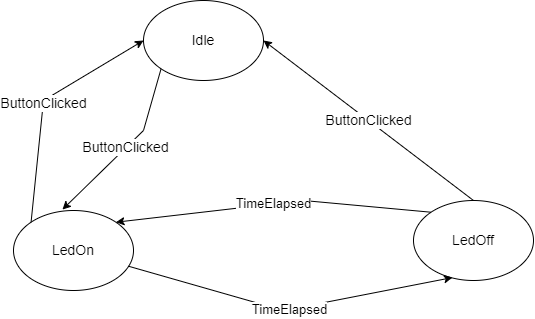
\includegraphics[width=0.85\textwidth]{img/blinking-led-state-machine.png}
    \caption{Stavový automat pre blikajúcu led žiarovku s možnosťou vypnutia pomocou tlačidla}
    \label{figure:blinking-led-state-machine}
\end{figure}

Stavový automat \textit{P} je teda definovaný ako pätica ($\Sigma$ ,$\mathcal{Q}$ , $q_0$, $\mathcal{F}$, $\delta$)
\begin{itemize}
    \item \begin{math} \Sigma = \{ \textit{ButtonClicked}, \textit{TimeElapsed} \}  \end{math}
    \item \begin{math} Q = \{ \textit{LedOn}, \textit{LedOff}, \textit{Idle} \}  \end{math}
    \item \begin{math} q_0 = \{ \textit{Idle} \}  \end{math}
    \item $\mathcal{F}$ \begin{math} = \{ \}  \end{math}
\end{itemize}
a prechodová funkcia $\delta$ je daná obrázkom \ref{figure:blinking-led-state-machine}.

\subsubsection{Implementácia stavového automatu}
Implementáciu začneme vytvorením niekoľkých globálnych premenných. Ako prvé definujeme enum stavov a enum udalostí definovaných v stavovom automate \textit{P}.
\begin{lstlisting}[
    label={lst:events-and-states},
    language=c++]  

enum States
{
    LedOn,
    LedOff,
    Idle
};

enum Events
{
    ButtonClicked,
    TimeElapsed,
};    

\end{lstlisting}
Interro definuje triedu \textit{StateMachine}. Pomocou tejto triedy vieme reprenzentovať stavový automat \textit{P} v našom programe. Trieda definuje jeden
parametrický konštruktor, ktorého argumentom je počiatočný stav automatu. Podľa definície \textit{P} to je stav \textit{Idle}. Vytvoríme preto inštanciu danej triedy s
názvom \textit{blinkingMachine} a nastavíme správny počiatočný stav automatu.
\begin{lstlisting}[
    label={lst:events-and-states},
    language=c++]  

StateMachine blinkingMachine(States::Idle);

\end{lstlisting}

Nasleduje definícia prechodovej funkcie automatu. V knižnici Interro sa prechodová funkcia definuje samostatne pre každý stav.
Definícia pre stav \textit{LedOn} vyzerá nasledovne:

\begin{lstlisting}[language=c++]  

static const int8_t ledOnStateTable[]{
    Events::ButtonClicked, States::Idle,
    Events::TimeElapsed, States::LedOff,
    -1};
    
\end{lstlisting}

Definícia je jednorozmerné pole, ktoré sa skladá z dvojíc udalostí a stavov. Táto dvojica reprezentuje prechod medzi stavmi. V prechodovej funkcii na obrázku číslo
\ref{figure:blinking-led-state-machine} vidíme, že zo stavu \textit{LedOn} sa vieme dostať do stavu \textit{Idle} ale aj do stavu \textit{LedOff}.
To aký bude ďalší stav definuje udalosť (vstupná abeceda), ktorá nastala. To vidíme aj v prechodovej tabuľke: Udalosť \textit{ButtonClicked} hovorí o prechode do stavu
\textit{Idle} a udalosť \textit{TimeElapsed} definuje prechod do stavu \textit{LedOff}. Pre čitateľnosť kódu je dôležité zvoliť správne formátovanie poľa.
Prechodová tabuľka stavu musí byť vždy ukončená číslom -1. Na základe toho implementácia Interro knižnice zistí veľkosť poľa a je schopná s ním vykonávať operácie.
Rovnakým spôsobom nadefinujeme prechodové tabuľky pre každý stav automatu \textit{P}:

\begin{lstlisting}[language=c++]  

static const int8_t idleStateTable[]{
    Events::ButtonClicked, States::LedOn,
    -1};

static const int8_t ledOnStateTable[]{
    Events::ButtonClicked, States::Idle,
    Events::TimeElapsed, States::LedOff,
    -1};

static const int8_t ledOffStateTable[]{
    Events::ButtonClicked, States::Idle,
    Events::TimeElapsed, States::LedOn,
    -1};
    
\end{lstlisting}

Definovali sme teda stavy, ktoré môže automat nadobudnúť. Rovnako aj udalosti spolu s prechodovými tabuľkami automatu.
Tu ukončíme definíciu globálnych premenných a pokračujeme v implementácii v Arduino funkcii setup(), ktorá je zavolaná jedenkrát pri štarte programu.
Pomocou definovaných globálnych premenných nakonfigurujeme spomínanú premennú \textit{blinkingMachine} typu \textit{StateMachine}. Konfigurácia funguje
na rovnakom princípe ako definícia prechodových tabuliek: každý stav automatu konfigurujeme samostatne. Konfigurácia pre náš príklad je nasledujúca:

\begin{lstlisting}[language=c++]  

blinkingMachine.configure(States::Idle)
    .onEvent(idleStateTable);

blinkingMachine.configure(States::LedOn)
    .onEvent(ledOnStateTable)
    .onEntry([](int8_t state)
            {
                TurnOnLed();
            });

blinkingMachine.configure(States::LedOff)
    .onEvent(ledOffStateTable)
    .onEntry([](int8_t state)
            { 
                TurnOffLed();
            });
        
    \end{lstlisting}

Ako prvé je vždy nutné zavolať metódu \textit{configure} (tento princíp sa opakuje v celej knižnici Interro).
Ako argument do metódy posielame stav, pre ktorý chceme konfiguráciu vykonať. Nasleduje volanie metódy \textit{onEvent}, tu ako argument posielame prechodovú tabuľku
stavu, ktorý konfigurujeme. Po volaní týchto dvoch metód je konfigurácie stavu hotová. Interro nám však umožnuje aj volanie vlastných metód pri vstupe a
výstupe zo stavu. V príklade vidíme volanie metódy  \textit{onEntry}. Do nej je možné poslať smerník na funkciu, prípadne lambda funckiu ako to vidíme
v príklade vyššie. Táto funkcia bude následne zavolaná vždy pri vstupe stavového automatu do konfigurovaného stavu. V našom príklade pri vstupe do stavu
\textit{LedOn} zavoláme funckiu \textit{TurnOnLed}, ktorá zasvieti led žiarovku. Analogicky pri vstupe do stavu \textit{LedOff}, voláme funckiu \textit{TurnOffLed},
ktorá led žiarovku zhasne. Rovnakým spôsobom funguje aj volanie metódy
\textit{onExit}. Jediným rozdielom je, že poskytnutá funkcia bude zavolaná pred opustením daného stavu. Túto možnosť však v našom príklade nevyužívame.

\subsubsection{Spúšťače udalostí}
V predchádzajúcej podkapitole sme namodelovali náš program pomocou stavového automatu a následne sme tento automat pomocou knižnice Interro aj implementovali.
Automat definuje stavy v ktorých sa môže nachádzať. Zároveň definuje aj prechody medzi stavmi a umožnuje volanie vlastných metód užívateľa pri zmene aktuálneho stavu.
Poslednou chýbajúcou časťou sú udalosti a ich spúšťanie. O to sa v Interro knižnici starajú takzvané spúšťače. \par
Spúšťače sú zodpovedné za sledovanie udalostí a ich následnú propagáciu do stavových automatov Interra. Delíme ich na dva druhy: hardvérové a softvérové spúšťače. \par
Hardvérový spúšťač používa na informovanie o udalosti prerušenia mikrokontroléra. Je napojený priamo na ISR prerušenia a obsahuje logiku pre konfiguráciu prerušení,
ktoré podporuje. \par
Príkladom hardvérového spúšťača je \textit{Timer1Trigger}. Využíva časovač číslo 1 mikrokontroléra Arduino Mega 2560 a podporuje rôzné módy.
Práve tento spúšťač použijeme na generovanie udalosti \textit{TimeElapsed}. Prvým krokom je vytvorenie ďalšej globálnej premennej typu \textit{Timer1Trigger}.
Pomenujeme ju ako \textit{timerTrigger}.
\begin{lstlisting}[language=c++]  
Timer1Trigger timerTrigger;            
\end{lstlisting}

Nasleduje konfigurácia spúšťača v Arduino funkcii setup:
\begin{lstlisting}[language=c++]  
timerTrigger.configure(TimerMode::CTC)
    .onTimeElapsed(1000, Events::TimeElapsed); 
\end{lstlisting}

Daným kódom konfigurujeme spúšťač, v našom konkrétnom prípade časovač 1, aby používal CTC mód, a po uplynutí každých 1000 milisekúnd oboznámil stavové automaty
o udalosti \textit{TimeElapsed}. \par

Druhým typom spúšťačov sú takzvané softvérove spúšťače. Pri hardvérových spúšťačoch je prvotným impulzom na vygenerovanie udalosti mikrokontrolér. Ten pomocou prerušenia
o tom oboznámi hardvérový spúšťač. Ak žiadne prerušenie nenastalo, spúšťač nevykonáva žiadnu akciu. Pri softvérových spúšťačoch to funguje inak. Interro knižnica
má zoznam všetkých softvérových spúšťačov a neustále sa na ne dopytuje či niektorá z udalosí nenastala. Ak spúštač odpovie definovanou udalosťou,
tak tá je rovnakým spôsobom preposlaná do všetkých zaregistrovaných stavových automatov. \par
V našom príklade využijeme ako softvérový spúšťač nazvaný ako \textit{ButtonTrigger}. Ako aj v predošlých prípadoch, prvým krokom je definovanie globálnej premennej
\textit{buttonTrigger} typu \textit{ButtonTrigger}.

\begin{lstlisting}[language=c++]  
ButtonTrigger buttonTrigger;            
\end{lstlisting}

Nasleduje konfigurácia spúšťača v Arduino funkcii setup:
\begin{lstlisting}[language=c++]  
buttonTrigger.configure(5)
    .onClick(Events::ButtonClicked); 
\end{lstlisting}

Spúšťač \textit{buttonTrigger} sme nakonfigurovali tak aby sledoval Arduino pin číslo 5 a v prípade stlačenia tlačidla pripojeného na tento pin, vygeneroval udalosť
\textit{ButtonClicked}. \par
Pre správnu funkčnosť celej knižnice je nakoniec nutné v Arduino funkcii \textit{loop} volať metódu \textit{run}, definovanú v globálnom kontajneri Interro knižnice.
\begin{lstlisting}[language=c++]  
void loop()
{
    interro.run();
}
\end{lstlisting}

\subsection{Implementovaná triggre}
\subsubsection{Timer trigger}

\subsubsection{External trigger}

\subsubsection{Pin change trigger}

\subsubsection{Soft triggers}
